\documentclass[aspectratio=169,10pt]{beamer}

\usepackage{amsmath}
\usepackage{booktabs}
\usepackage{graphicx}
\usepackage{array}
\usepackage{xcolor}

\graphicspath{{figures/}}

\definecolor{LMBlue}{HTML}{2684FC}
\definecolor{LMGreen}{HTML}{00AC47}
\definecolor{LMYellow}{HTML}{FBBC04}
\definecolor{LMRed}{HTML}{EA4335}
\definecolor{LMPurple}{HTML}{A142F4}
\definecolor{LMLight}{HTML}{F5F8FC}
\definecolor{LMDark}{HTML}{202124}
\definecolor{LMMuted}{HTML}{5F6368}

\setbeamercolor{normal text}{fg=LMDark,bg=white}
\setbeamercolor{structure}{fg=LMBlue}
\setbeamercolor{frametitle}{fg=white,bg=LMBlue}
\setbeamercolor{title}{fg=LMBlue}
\setbeamercolor{subtitle}{fg=LMMuted}
\setbeamercolor{block title}{fg=white,bg=LMBlue}
\setbeamercolor{block body}{fg=LMDark,bg=LMLight}
\setbeamercolor{alerted text}{fg=LMRed}
\setbeamerfont{frametitle}{series=\bfseries,size=\large}
\setbeamerfont{title}{series=\bfseries,size=\LARGE}
\setbeamerfont{subtitle}{size=\large}
\setbeamertemplate{navigation symbols}{}
\setbeamertemplate{itemize item}{\color{LMBlue}$\blacktriangleright$}
\setbeamertemplate{itemize subitem}{\color{LMGreen}$\bullet$}
\setbeamertemplate{footline}{
  \leavevmode
  \hbox{
    \begin{beamercolorbox}[wd=.82\paperwidth,ht=3.0ex,dp=1.7ex,leftskip=1em]{author in head/foot}
      \color{LMMuted}\scriptsize LMPool: Locality-Aware Routing and NVLink KV-Cache Transfer
    \end{beamercolorbox}
    \begin{beamercolorbox}[wd=.18\paperwidth,ht=3.0ex,dp=1.7ex,rightskip=1em plus1fil]{date in head/foot}
      \color{LMMuted}\scriptsize \insertframenumber/\inserttotalframenumber
    \end{beamercolorbox}
  }
  \vskip0.3em
}

\newcommand{\sys}{LMPool}
\newcommand{\metric}[1]{\textcolor{LMBlue}{\bfseries #1}}
\newcommand{\good}[1]{\textcolor{LMGreen}{\bfseries #1}}
\newcommand{\caution}[1]{\textcolor{LMRed}{\bfseries #1}}

\title{\sys{}}
\subtitle{Locality-Aware Routing and NVLink KV-Cache Transfer for Multi-GPU LLM Serving}
\author{Jialiang Li}
\institute{The Hong Kong University of Science and Technology}
\date{July 28th 2026}

\begin{document}

\begin{frame}[plain]
  \titlepage
  \vspace{-1.2em}
  \begin{center}
    \small\url{https://github.com/0x0addc001/LMPool}
  \end{center}
\end{frame}

\begin{frame}{The Placement Mismatch}
  \begin{columns}[T,onlytextwidth]
    \begin{column}{0.48\textwidth}
      \begin{block}{What prefix caching assumes}
        Reuse is cheap when a request executes where its KV prefix already resides.
      \end{block}
      \vspace{0.4em}
      \begin{block}{What data parallelism does}
        Each GPU owns an independent allocator and physical KV cache, while ingress assigns requests globally.
      \end{block}
    \end{column}
    \begin{column}{0.48\textwidth}
      \begin{itemize}
        \item Round robin may send a matching request to the wrong GPU.
        \item Strict owner routing can overload one replica.
        \item Unconditional KV movement can cost more than recomputation.
      \end{itemize}
      \vspace{0.5em}
      \begin{alertblock}{Design question}
        When should the system route to existing KV, and when should KV move to demand?
      \end{alertblock}
    \end{column}
  \end{columns}
\end{frame}

\begin{frame}{Two Principles}
  \begin{columns}[T,onlytextwidth]
    \begin{column}{0.48\textwidth}
      \begin{block}{Routing Principle: Cache Locality}
        Send a request to a GPU that already owns the longest useful contiguous prefix when the saved prefill work exceeds queueing and capacity pressure.
      \end{block}
      \vspace{0.5em}
      \begin{center}
        \Large\good{Route before transfer}
      \end{center}
    \end{column}
    \begin{column}{0.48\textwidth}
      \begin{block}{Transfer Principle: Cache Fluidity}
        Copy or move complete KV block chains over a direct NVLink pair when cache placement no longer matches future demand and expected reuse repays the transaction.
      \end{block}
      \vspace{0.5em}
      \begin{center}
        \Large\good{Transfer only when profitable}
      \end{center}
    \end{column}
  \end{columns}
  \vspace{0.8em}
  \begin{center}
    \large \metric{Avoid recomputation without turning locality into a load hotspot}
  \end{center}
\end{frame}

\begin{frame}{System Architecture}
  \begin{center}
    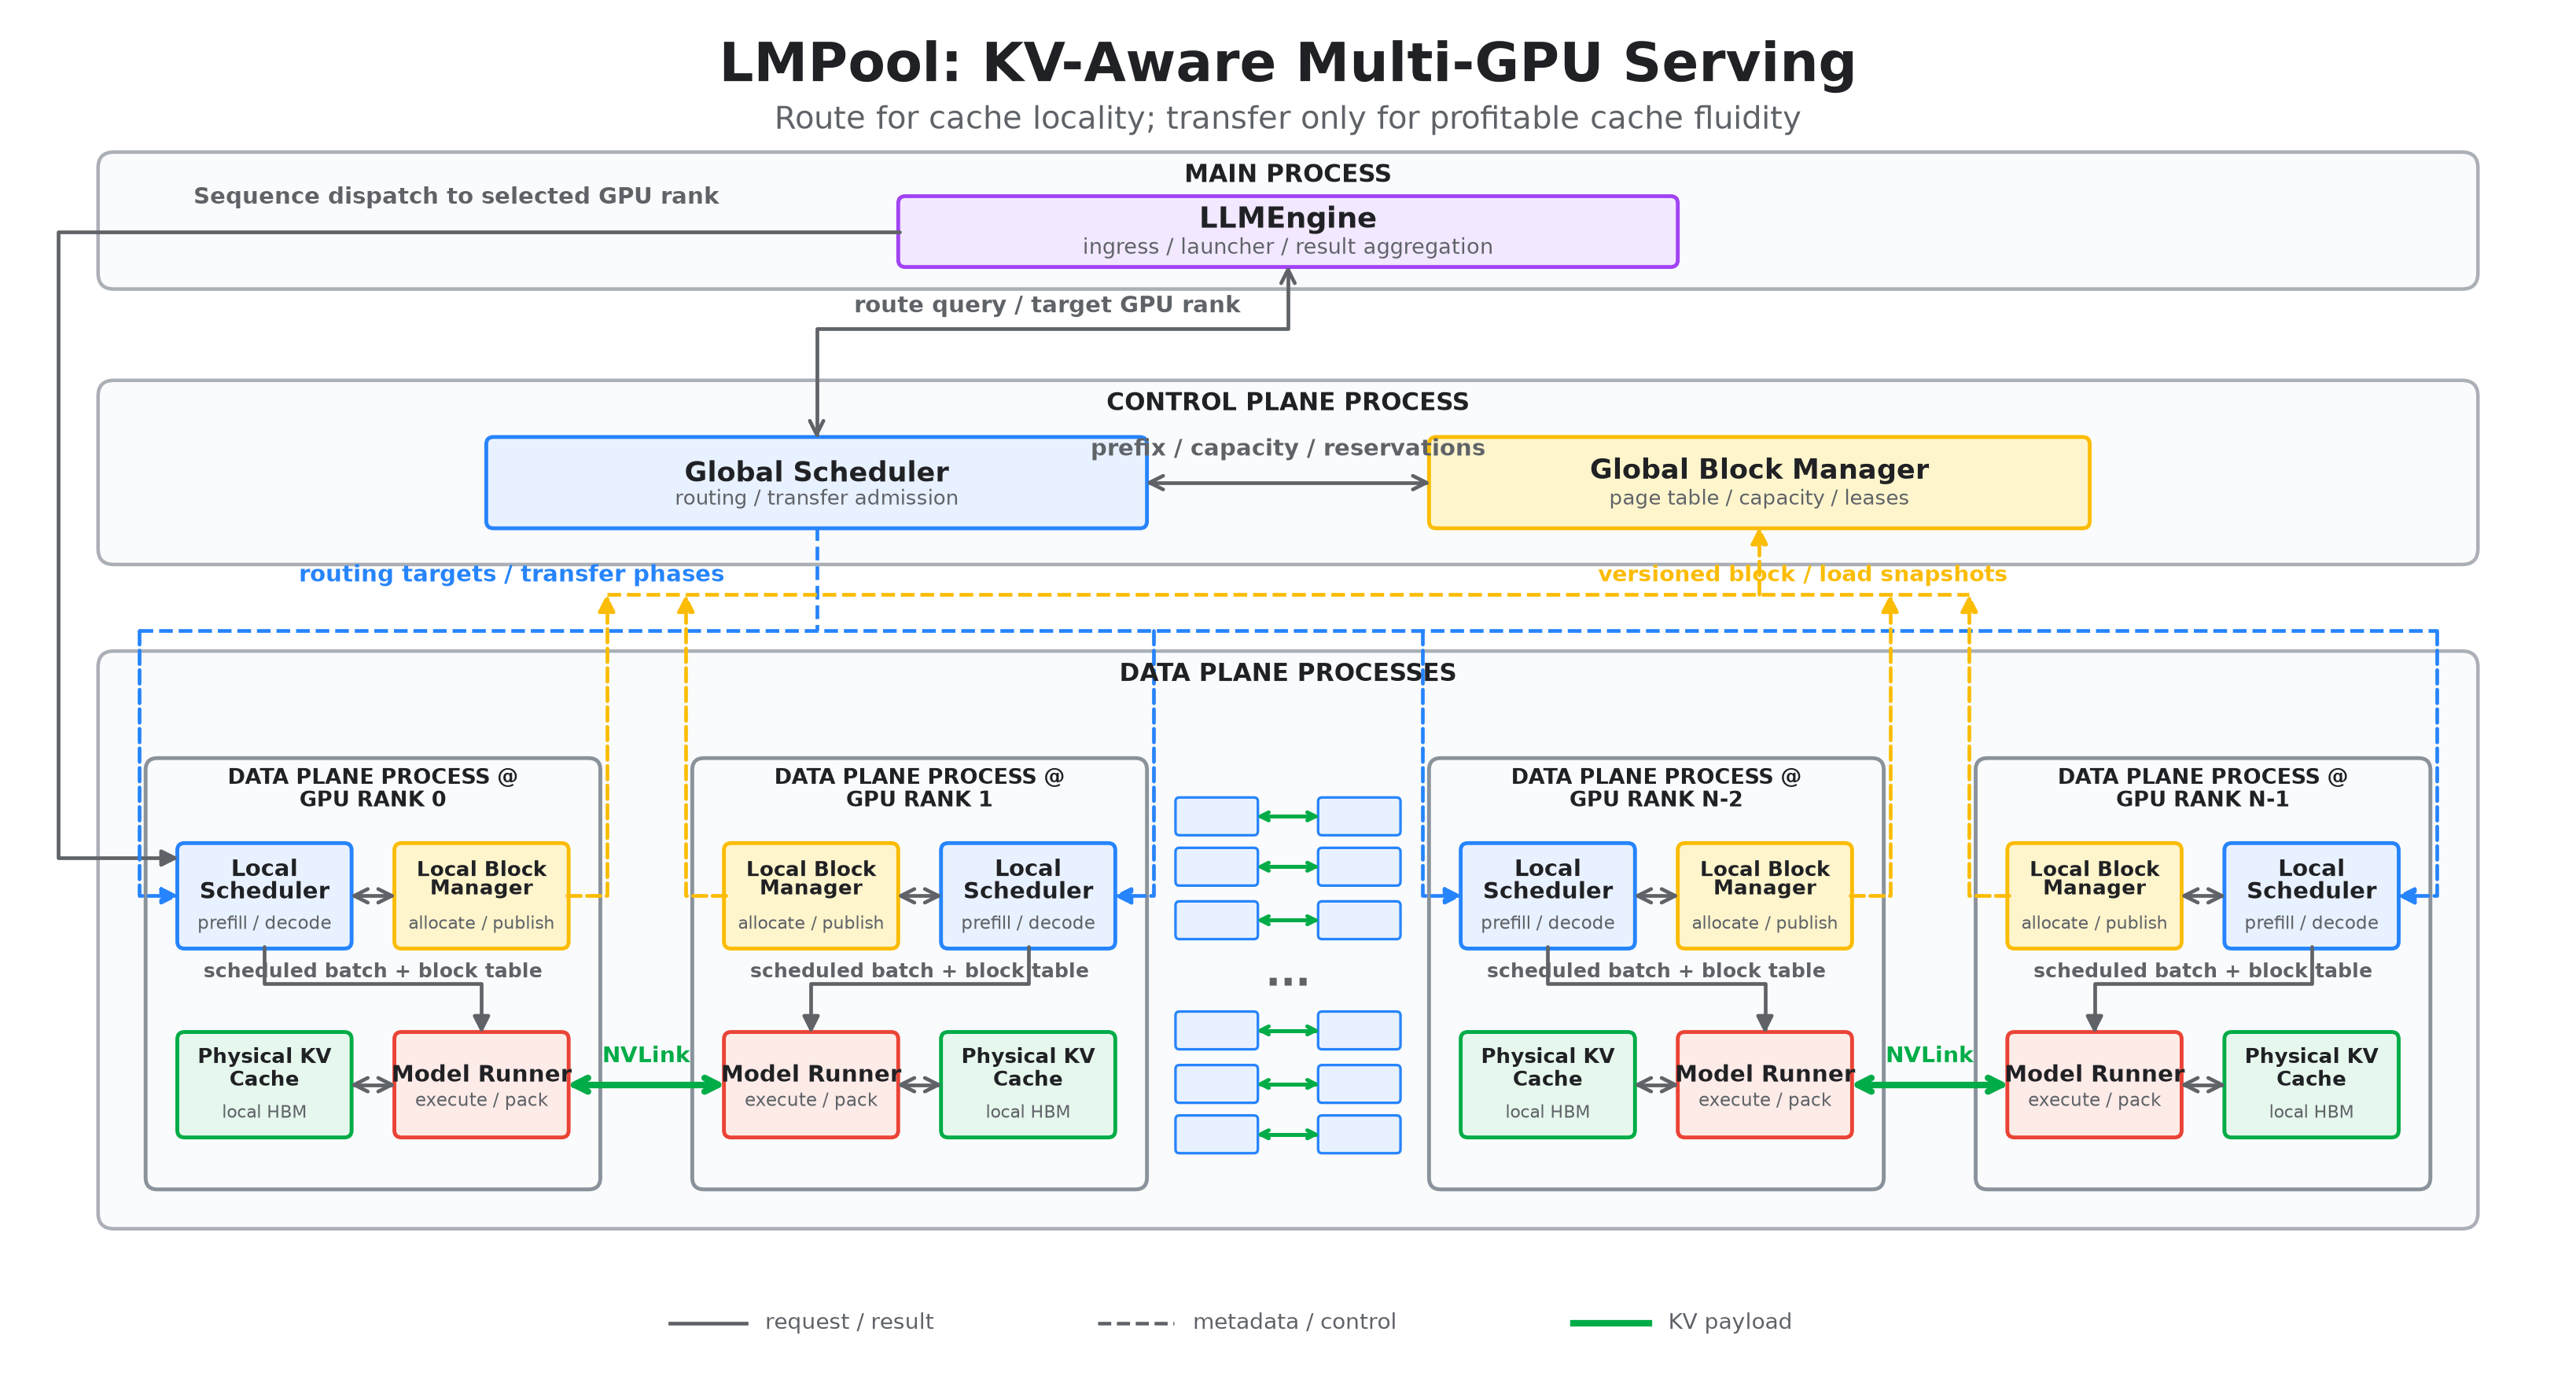
\includegraphics[width=0.95\textwidth,height=0.78\textheight,keepaspectratio]{fig_architecture.png}
  \end{center}
\end{frame}

\begin{frame}{A Request Through \sys{}}
  \small
  \begin{enumerate}
    \item \metric{Ingress:} LLMEngine tokenizes the prompt, builds a Sequence, and computes chained hashes for complete prompt blocks.
    \item \metric{Global route:} Global Scheduler reads versioned prefix, load, and capacity metadata and reserves the selected rank.
    \item \metric{Local admission:} The target Local Scheduler reuses ready local blocks and asks Local Block Manager to allocate missing blocks.
    \item \metric{Optional foreground transfer:} A real block shortage may trigger a cost-gated pair-local copy or move plan.
    \item \metric{Execution:} Model Runner performs prefill, writes missing KV, and then iterates decode.
    \item \metric{Publication:} The worker reports tokens and a new versioned block/load snapshot, only ready blocks become globally visible.
    \item \metric{Completion:} References are released. Complete prefixes remain cached at ref-count zero until reuse or dependency-safe reclamation.
  \end{enumerate}
\end{frame}

\begin{frame}{KV-Aware Routing}
  \begin{columns}[T,onlytextwidth]
    \begin{column}{0.49\textwidth}
      \small
      For candidate GPU $g$:
      \begin{align*}
        n_g &= \max(0,R-h_g),\\
        M_g &= \min(N,n_gS),\\
        A_g &= \max(0,n_g-F_g),\\
        C_{\mathrm{route}}(g) &= Q_g + w_pM_g + w_eA_gS.
      \end{align*}
      \vspace{-0.5em}
      \begin{alertblock}{Decision}
        Select the feasible rank with minimum projected token-equivalent work.
      \end{alertblock}
    \end{column}
    \begin{column}{0.47\textwidth}
      \scriptsize
      \begin{itemize}
        \item $R$: required prompt blocks, $N$: prompt tokens
        \item $S$: tokens per block, $h_g$: contiguous ready blocks
        \item $n_g$: missing blocks, $M_g$: missing prefill tokens
        \item $F_g$: currently free blocks
        \item $A_g$: missing blocks beyond $F_g$, hence reclaim pressure
        \item $Q_g$: queued, pending, and running token-equivalent work
        \item $w_p,w_e$: prefill and reclaim cost weights
      \end{itemize}
      \vspace{0.1em}
      \begin{block}{Bounded spill}
        Bypass an overloaded owner only when additional recomputation remains bounded.
      \end{block}
    \end{column}
  \end{columns}
\end{frame}

\begin{frame}{Transactional KV Transfer}
  \begin{center}
    
\includegraphics[width=0.94\textwidth,height=0.74\textheight,keepaspectratio]{fig_kv_block_lifecycle.png}
  \end{center}
  \vspace{-0.5em}
  \begin{center}
    \small Prepare $\rightarrow$ Execute $\rightarrow$ Publish $\rightarrow$ Finalize,
    abort preserves the source and releases the destination reservation.
  \end{center}
\end{frame}

\begin{frame}{Cost-Gated Transfer Admission}
  \begin{center}
    
\includegraphics[width=0.94\textwidth,height=0.72\textheight,keepaspectratio]{fig_transfer_cost_model.png}
  \end{center}
  \vspace{-0.5em}
  \begin{center}
    \small Static cost uses the pair-specific P95 profile plus a calibrated residual.
    Fixed latency is only a zero-default fallback, completed plans update EWMA residuals.
  \end{center}
\end{frame}

\begin{frame}{Evaluation Design}
  \small
  \begin{columns}[T,onlytextwidth]
    \begin{column}{0.45\textwidth}
      \begin{itemize}
        \item 6 RTX 3090 GPUs, 3 direct NV4 pairs
        \item Qwen3-0.6B and Qwen3-1.7B, BF16
        \item Same per-worker KV budget
        \item 5 trials, fixed seed, EOS disabled
        \item Outputs: routing 64, memory skew 16, load skew 8 tokens
        \item Controlled internal ablations
      \end{itemize}
    \end{column}
    \begin{column}{0.52\textwidth}
      \begin{tabular}{@{}p{0.31\linewidth}p{0.62\linewidth}@{}}
        \toprule
        Workload & Purpose \\
        \midrule
        Routing & 1x/3x/5x shared-prefix locality \\
        Load skew & Background copy plus placement leases \\
        Memory skew & Move-style capacity release \\
        \bottomrule
      \end{tabular}
    \end{column}
  \end{columns}
  \vspace{0.8em}
  \begin{alertblock}{Scope}
    Synthetic mechanism study, not a production-trace or production-engine comparison.
  \end{alertblock}
\end{frame}

\begin{frame}{Routing: Longer Prefixes Create Stable Gains}
  \begin{center}
    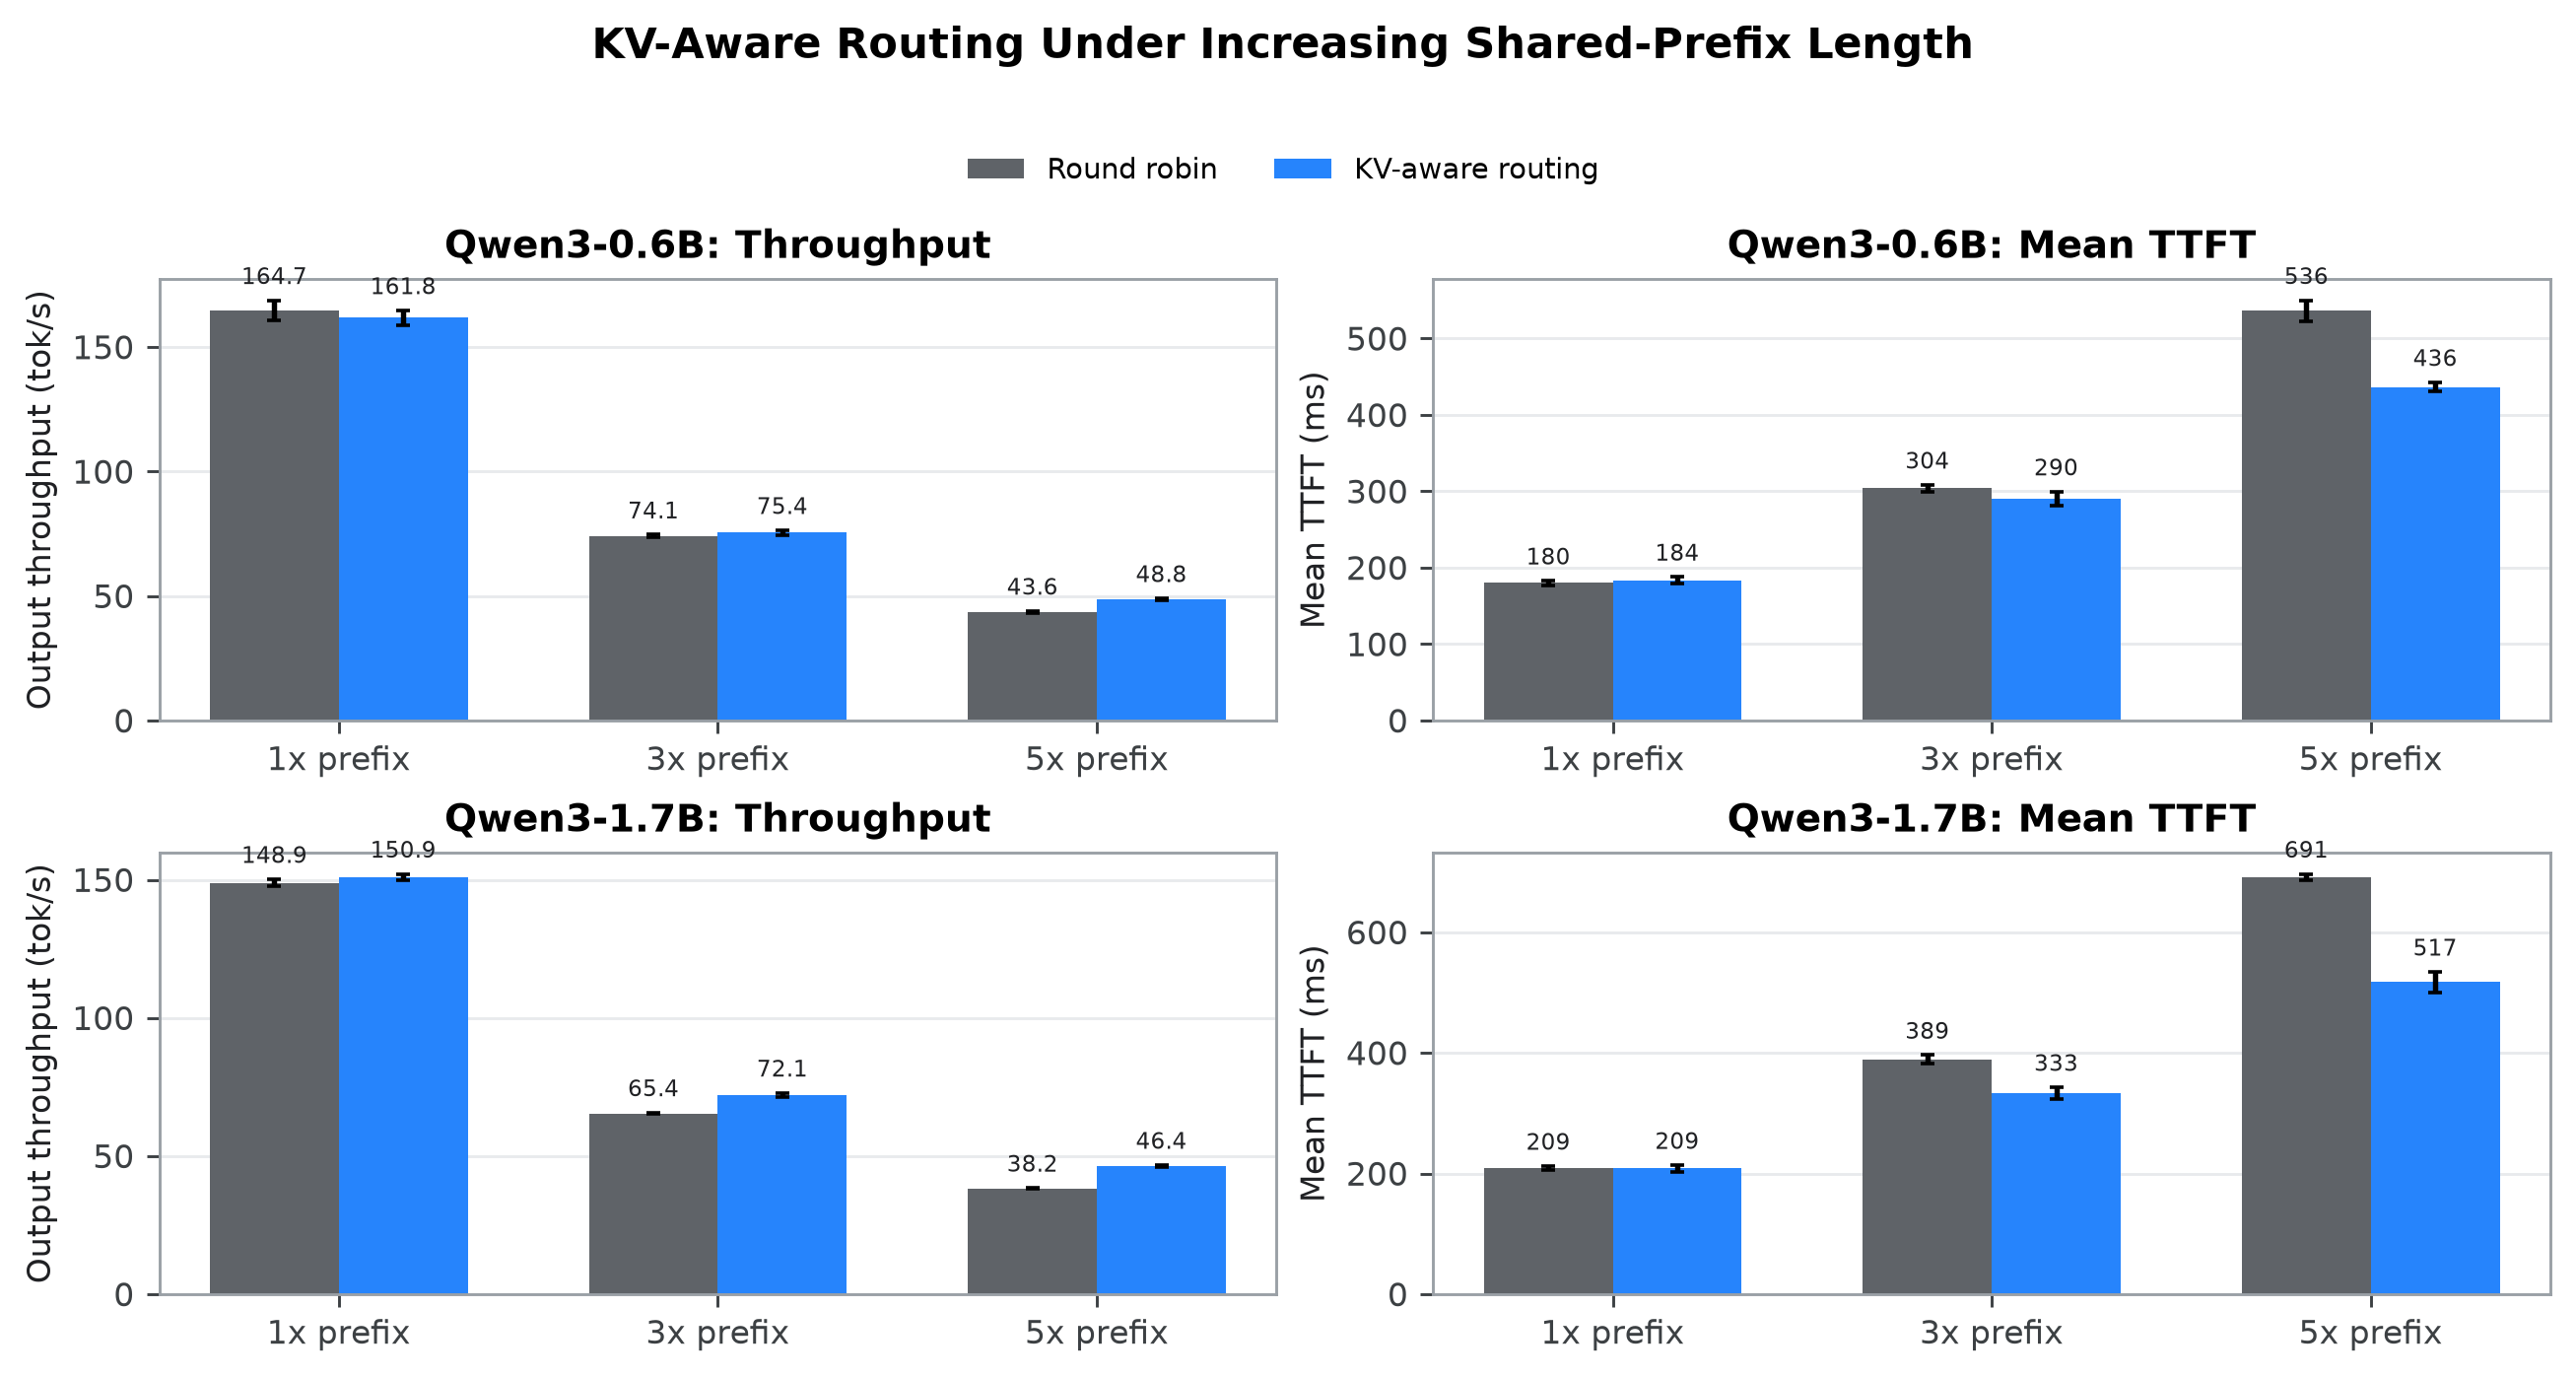
\includegraphics[width=0.94\textwidth,height=0.69\textheight,keepaspectratio]{fig_suite_routing.png}
  \end{center}
  \vspace{-0.5em}
  \begin{center}\small At 5x, routing improves throughput by \good{11.8\% / 21.3\%} and reduces TTFT by \good{18.6\% / 25.2\%} for 0.6B / 1.7B.\end{center}
\end{frame}

\begin{frame}{NVLink Data-Path Calibration}
  \begin{center}
    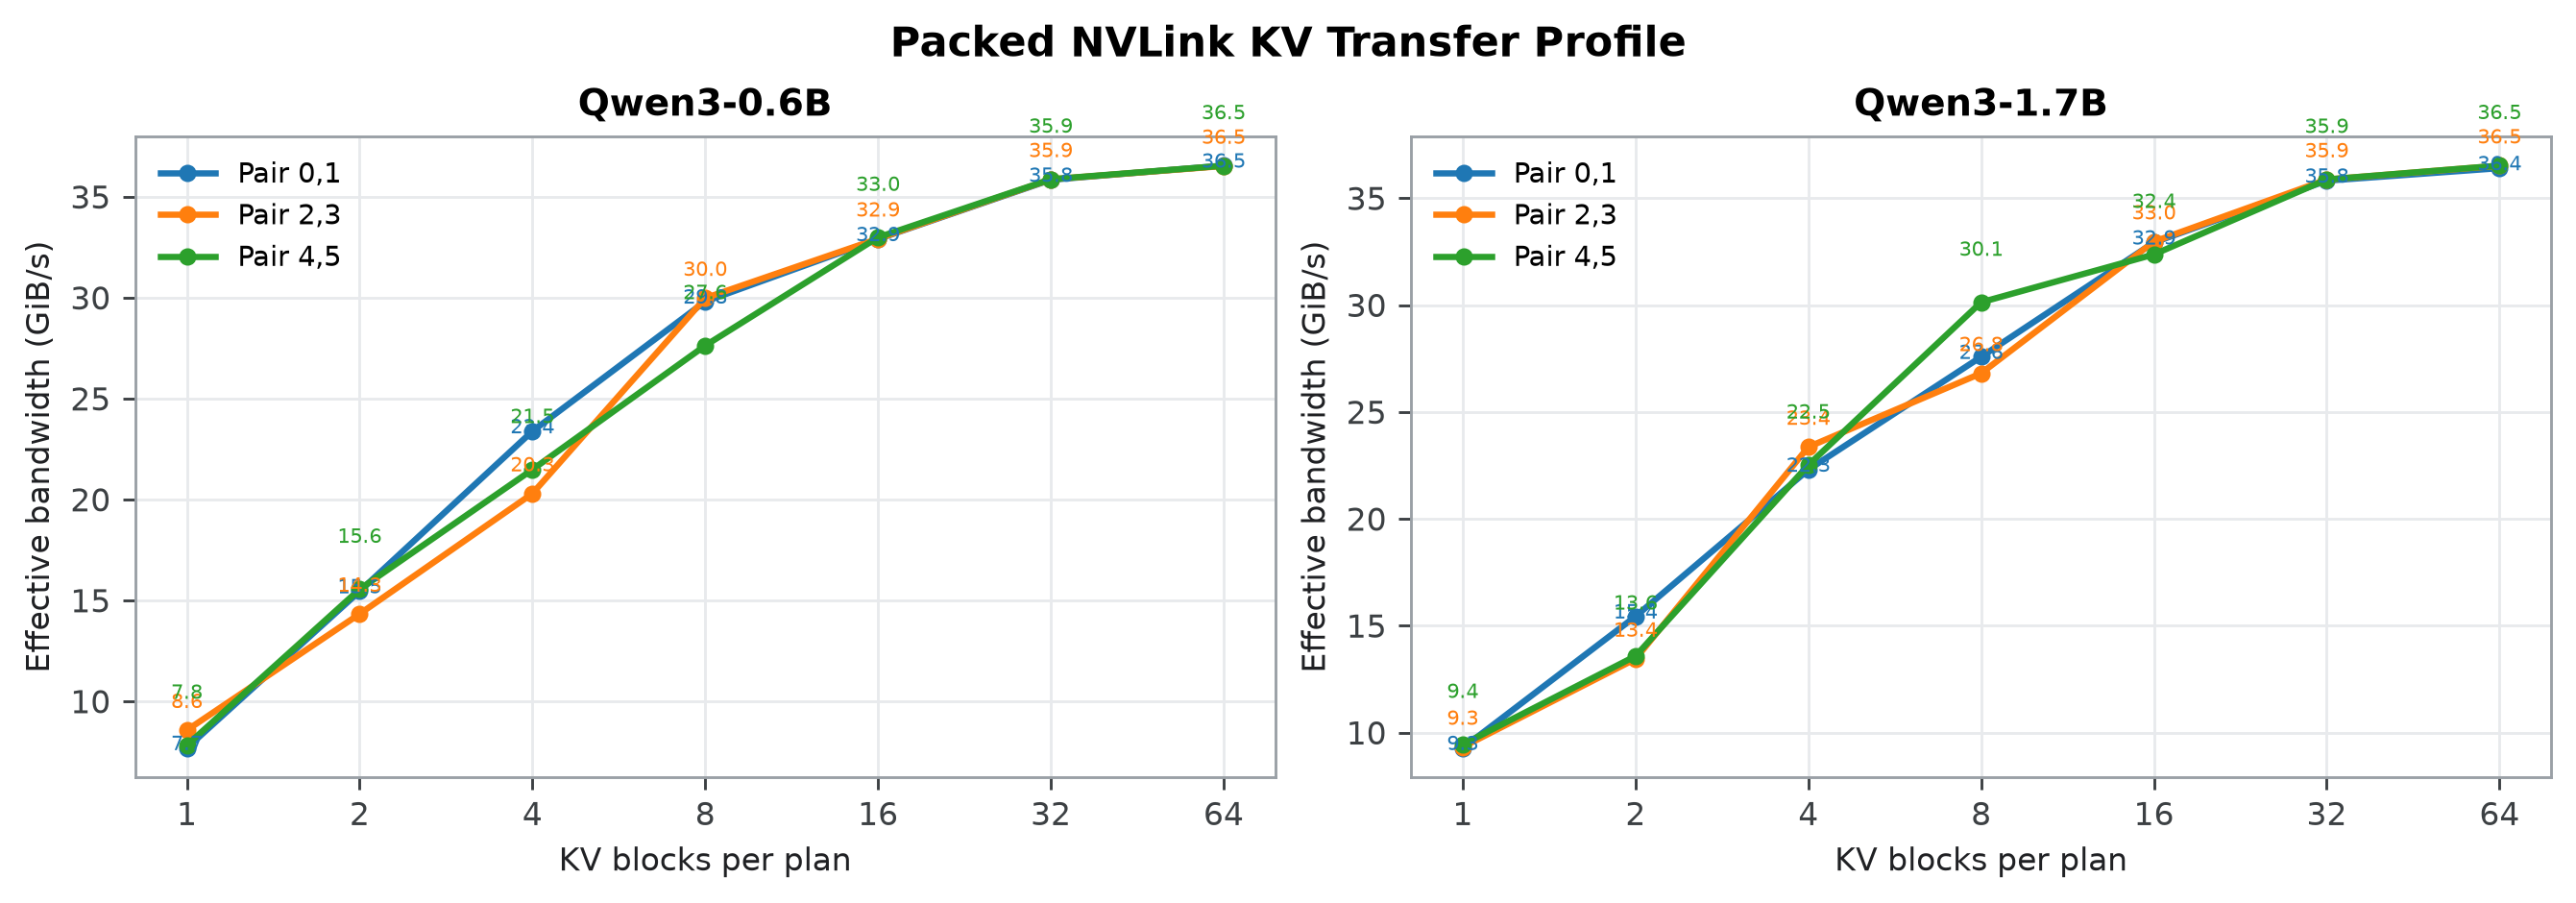
\includegraphics[width=0.94\textwidth,height=0.68\textheight,keepaspectratio]{fig_suite_transfer_profile.png}
  \end{center}
  \begin{alertblock}{Interpretation}
    Every destination passed byte validation. The 1-64 block curves calibrate the pair-specific cost model, they do not alone prove serving benefit.
  \end{alertblock}
\end{frame}

\begin{frame}{Transfer: Mechanism Evidence and Boundary}
  \begin{center}
    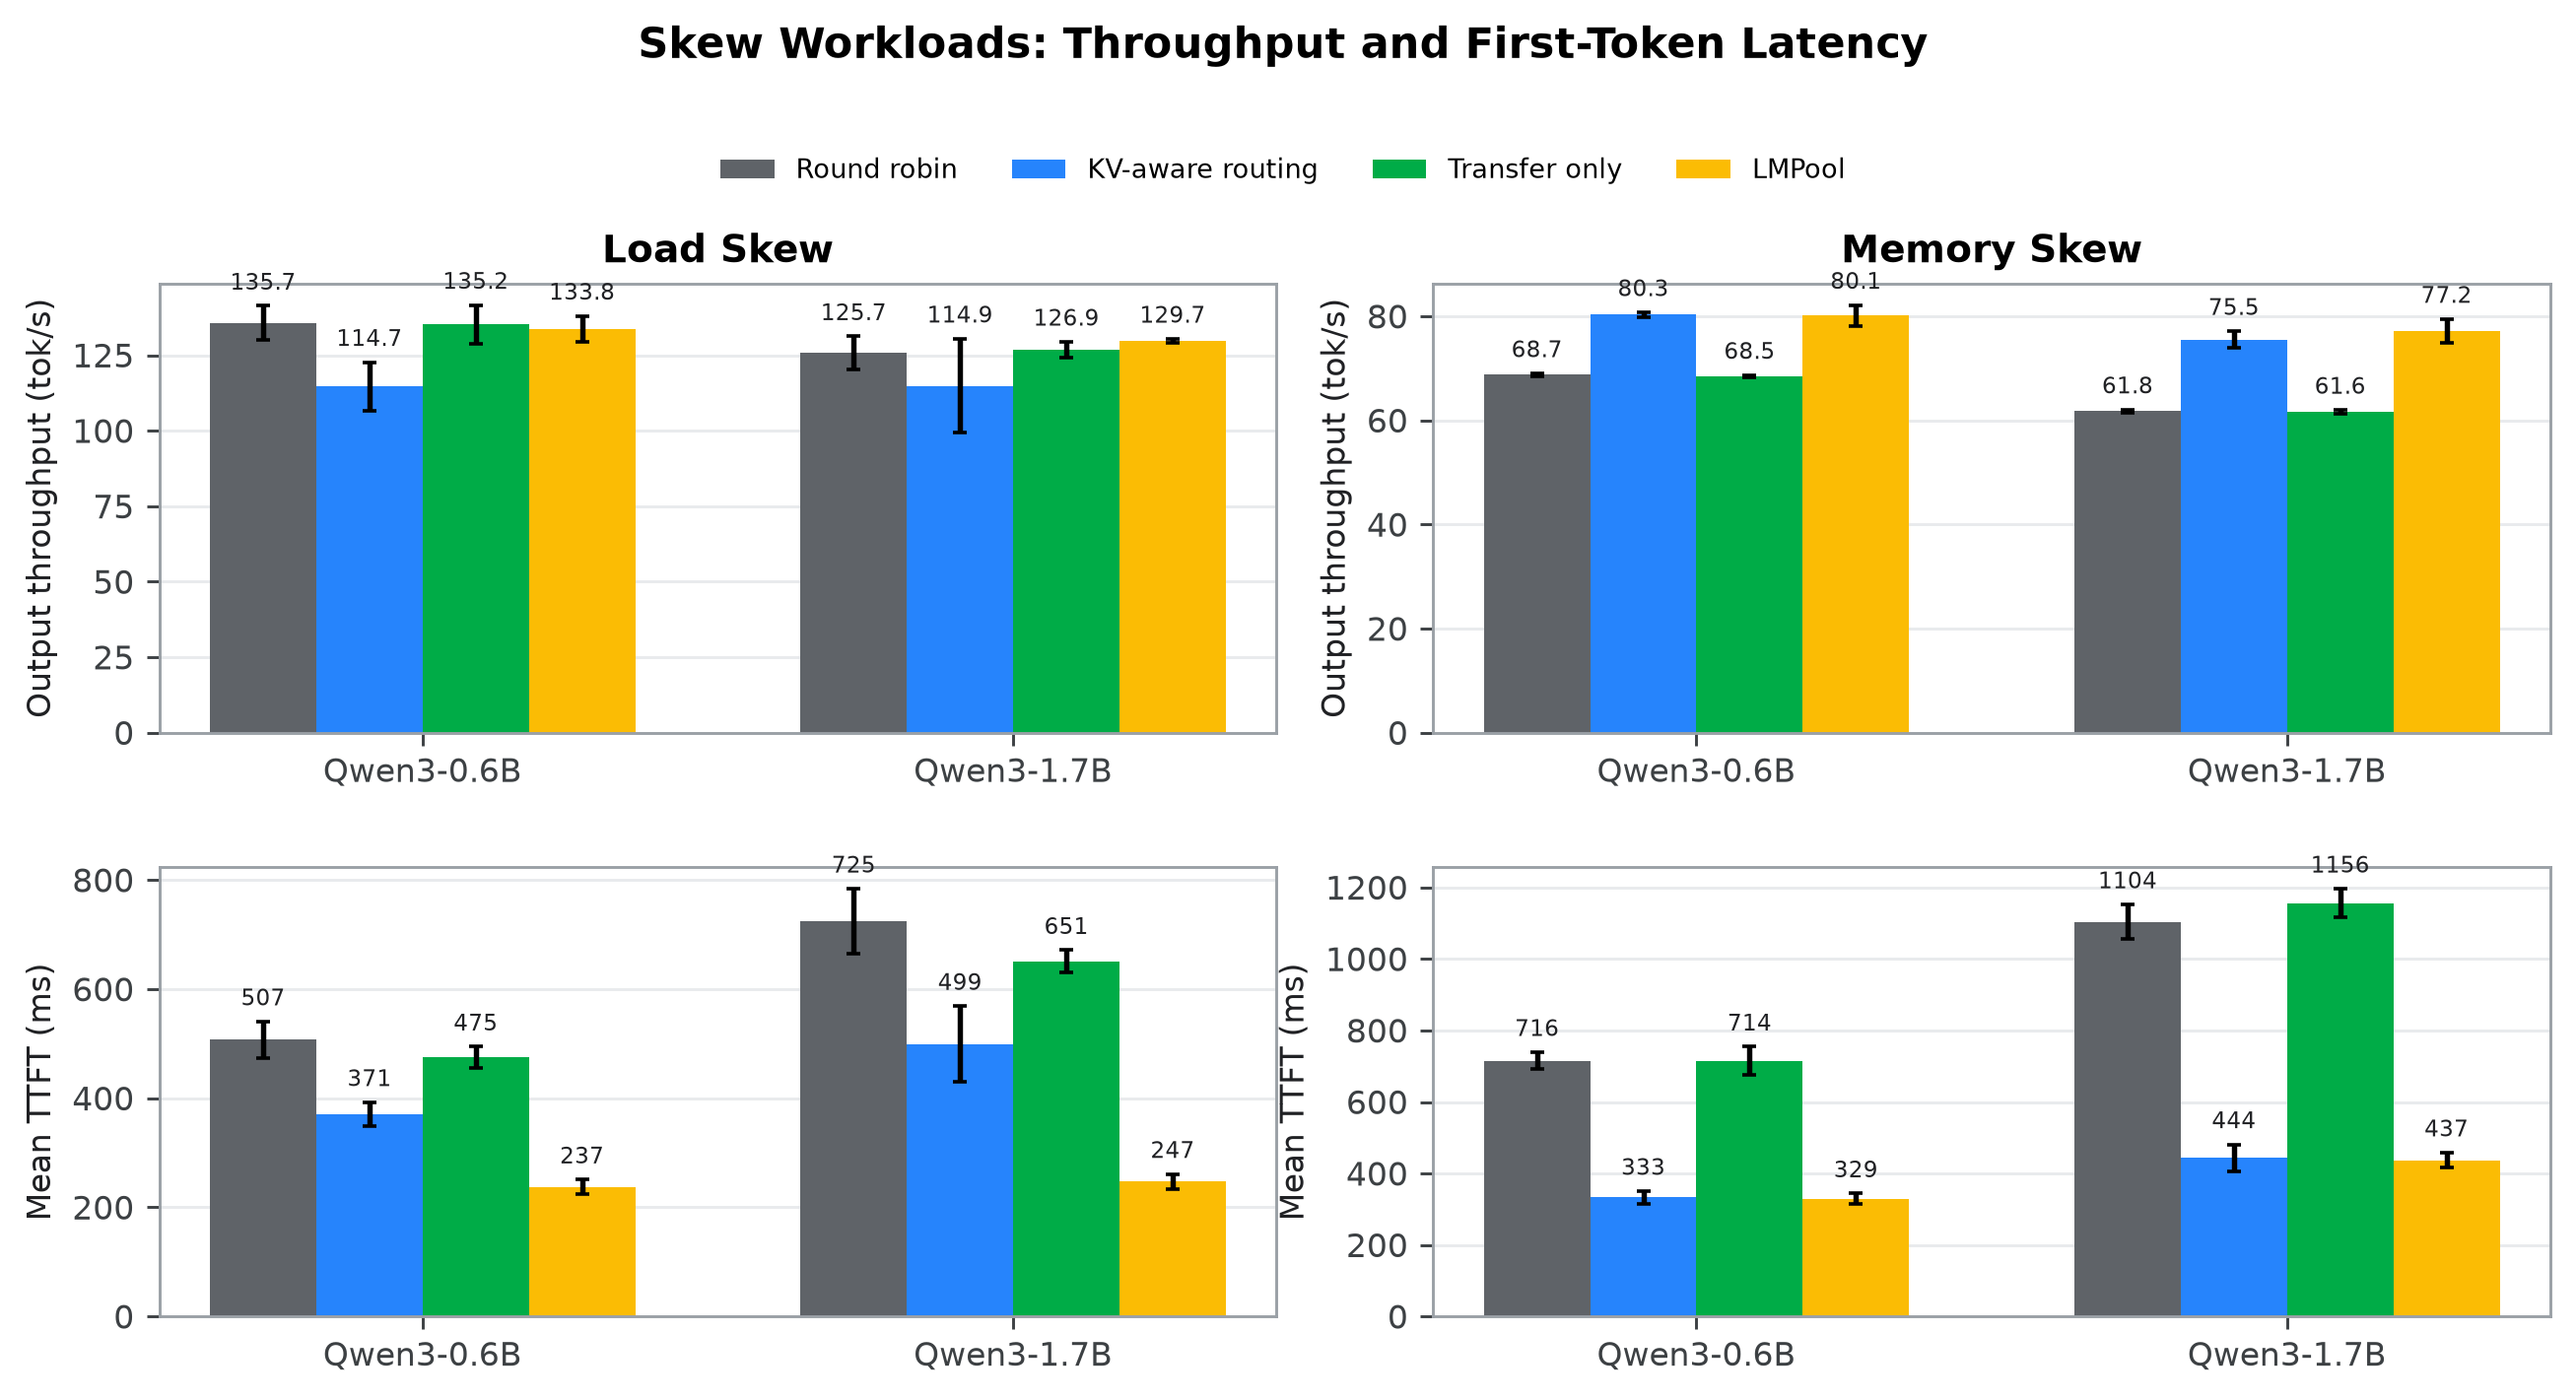
\includegraphics[width=0.94\textwidth,height=0.67\textheight,keepaspectratio]{fig_suite_skew.png}
  \end{center}
  \vspace{-0.55em}
  \begin{columns}[T,onlytextwidth]
    \begin{column}{0.48\textwidth}\small
      \good{Load skew:} three background placements copy 87 blocks. Placement leases serve 95 later requests. TTFT falls sharply, but a higher TPOT can offset mean E2E.
    \end{column}
    \begin{column}{0.48\textwidth}\small
      \caution{Memory skew:} 0.6B verifies 35 released source blocks. It remains close to routing-only, the 1.7B run does not satisfy the full offload verification predicate.
    \end{column}
  \end{columns}
\end{frame}

\begin{frame}{Limitations and Future Work}
  \small
  \begin{itemize}
    \item Synthetic workloads and deterministic replay order, no production trace evaluation
    \item Internal ablations rather than production-engine comparisons
    \item Six RTX 3090 GPUs, two sub-2B models with identical KV geometry
    \item No NVSwitch-fabric evaluation; pair-local profiles do not capture all-to-all target selection or shared-fabric contention
    \item Fixed 256-token block size, no block-size sensitivity study
    \item Pair-specific P95 profiles and online residuals, no held-out cost-prediction error or policy ablation
    \item Single control process and launcher, no consensus or launcher failover
  \end{itemize}
  \vspace{0.5em}
  \begin{block}{Next evaluation}
    Production traces and baselines, 1/2/4/6-GPU and block-size scaling, cost-model prediction and admission ablations, concurrent transfer profiles and end-to-end scaling on an eight-GPU NVSwitch domain.
  \end{block}
\end{frame}

\begin{frame}{Takeaways}
  \begin{enumerate}
    \item \metric{Routing solves cache locality:} reuse KV where it already resides without creating a load hotspot.
    \item \metric{NVLink transfer provides cache fluidity:} move complete block chains only when reuse repays the full transaction.
    \item \metric{Transfer mechanisms are verified in functionality but not performance:} background placement and foreground offloading execute under their respective stressors. However, a completed transfer does not automatically improve mean E2E or throughput.
  \end{enumerate}
  \vspace{1em}
  \begin{center}
    \Large\good{Route when possible. Transfer when profitable.}
  \end{center}
  \vfill
  \begin{center}
    \small Source: \url{https://github.com/0x0addc001/LMPool}
  \end{center}
\end{frame}

\begin{frame}[plain]
  \begin{center}
    \vspace{1.0em}
    {\color{LMBlue}\Huge\bfseries Thank You for Listening!}

    \vspace{1.4em}
    {\Large\color{LMBlue}\bfseries Questions?}

    \vspace{3em}
    {\Large Acknowledgments}

    \vspace{1em}
    \begin{minipage}{0.72\textwidth}
      \centering
      Thank Prof. Kai Chen and Yijun Sun for their guidance and feedback.
    \end{minipage}

    \vfill
    \small
    Jialiang Li \quad The Hong Kong University of Science and Technology

    \vspace{0.35em}
    \url{https://github.com/0x0addc001/LMPool}
  \end{center}
\end{frame}

\end{document}
